\documentclass[12pt,twoside]{article}
\usepackage[dvipsnames]{xcolor}
\usepackage{tikz,graphicx,amsmath,amsfonts,amscd,amssymb,bm,cite,epsfig,epsf,url}
\usepackage[hang,flushmargin]{footmisc}
\usepackage[colorlinks=true,urlcolor=blue,citecolor=blue]{hyperref}
\usepackage{amsthm,multirow,wasysym,appendix}
\usepackage{array,subcaption} 
% \usepackage[small,bf]{caption}
\usepackage{bbm}
\usepackage{pgfplots}
\usetikzlibrary{spy}
\usepgfplotslibrary{external}
\usepgfplotslibrary{fillbetween}
\usetikzlibrary{arrows,automata}
\usepackage{thmtools}
\usepackage{blkarray} 
\usepackage{textcomp}
\usepackage{pdfpages}
\usepackage[left=0.8in,right=1.0in,top=1.0in,bottom=1.0in]{geometry}
\newcommand{\rnd}{\Tilde  }
\newcommand{\rx}{\rnd{ x}  }
\newcommand{\ra}{\rnd{ a}  }
\newcommand{\ru}{\rnd{ u}  }
\newcommand{\rd}{\rnd{ d}  }
%\newcommand{\rs}{\rnd{ s}  }
\newcommand{\ri}{\rnd{ i}  }
\newcommand{\re}{\rnd{ e}  }
\newcommand{\rQ}{\rnd{ q}  }
\newcommand{\rC}{\rnd{ c}  }


\begin{document}

\begin{center}
{\large{\textbf{Homework 8}} } \\%\vspace{0.2cm}\\
Due November 21 at 11 pm
\\
\end{center}

\begin{enumerate}

\item (Short questions) 
\begin{enumerate}
\item Give an example of a nonnegative random variable $\ra$ and a constant $c > 0$ for which $P\{\ra \geq c\} = \E\brac{ \ra }/c$. What does this say about Markov's inequality?
\subitem
For our example, lets use a non-negative bernoulli random variable, let's call it $\ra$, who's pdf is defined in the following way:
$$
    \begin{cases}
    \ra = 1 & with \ P(\theta) \\
    \ra = 0 & with \ P(1-\theta)
    \end{cases}
$$
With $c=1$. Then what we would have is the following inequality:
$$
    P(\ra \geq c) \leq \frac{E(\ra)}{c} \longrightarrow 1 \leq 1 
$$
Since we have equality in the example we have used, there is no better bound than Markov's inequality.

\item In the notes, we have defined the sample variance of a dataset $X := \keys{x_1, x_2, \ldots, x_n}$ as
 \begin{align}
\sigma_{X}^2 &:= \frac{ \sum_{i=1}^{n}  (x_i - \mu_X)^2}{n},
\end{align}
where $\mu_X$ is the sample mean. Show that this is not an unbiased estimator of the true variance if the data are i.i.d. samples from a distribution with zero mean and variance $\sigma^2$. Explain how to fix the estimator so that it is unbiased.
\end{enumerate}
\subitem Intuitively, we understand that the samples we derive from a distribution of i.i.d. variables will always be subject to randomness and thus noise. Therefore, no matter what, the sample variance will be a biased estimator of the true population variance. We can show this by taking the expected value and expanding our initial equation, and doing a few math tricks to illustrate how it does not equal the true population variance of $\sigma^2$.

\begin{equation}
    \begin{split}
        E(\sigma_{X}^2) &= E(\frac{ \sum_{i=1}^{n}  (x_i - \mu_X)^2}{n}) \\
        E(\sigma_{X}^2) &= \frac{1}{n} \times E(\sum_{i=1}^n (x_i^2-2\mu_Xx_i + \mu_x^2))\\
        E(\sigma_{X}^2) &= \frac{1}{n}(E(x_i^2 + n\mu_X^2 - 2n\mu_X^2))\\
         E(\sigma_{X}^2) &= \frac{1}{n}((\simga_X^2 + \mu^2)-n(\frac{\sigma_X^2}{n}+\mu_X^2)) \\
         E(\sigma_{X}^2) &=\frac{1}{n}(n\sigma_X^2 - \sigma_X^2)\\
         \sigma_X^2 &\neq \sigma_X^2 - \frac{\simga_X^2}{n} \qed
    \end{split}
\end{equation}

We could divide our initial equation by $n-1$ instead of $n$ and it would yield: $$
    \frac{1}{n-1} \times (n-1) \times \sigma_X^2 = \sigma_X^2
$$
and thus would unbias our estimator.

\item (Poll) In an online poll before an election, 60 participants intend to vote for the Democratic candidate, and the remaining 40 intend to vote for the Republican candidate.  
\begin{enumerate}
\item The number of young people (between 18 and 35 years old) in the poll is 70. 50 intend to vote for the Democratic candidate. The fraction of young people among voters in general is 25\%. Provide an estimate of the proportion of voters that will vote for the Democratic candidate. 
\subitem
For the whole population we will have:
$$
    (\frac{1}{4} \times \frac{5}{7} ) + (\frac{3}{4} \times \frac{1}{3}) = \frac{3}{7}
$$
Who will vote Democrat.
\item Under what assumptions is your estimate unbiased? Justify your answer mathematically.
\subitem
The estimate will only be unbiased if within the two groups we have defined our population: young and not young, each behave and are sampled in i.i.d. fashion, that is to say they will have uniform likelihood and are sampled with replacement. Since we understand the proportions of young and not young voters in our population, we need to ensure that we get an unbiased estimate of the proportion of each group that votes democrat.
\item Let $\alpha$ be the proportion of young people in the population, $\theta_1$ the proportion of young people who vote for the Democratic candidate, and  $\theta_2$ the proportion of old people who vote for the Democratic candidate. If the number of young people in a poll is $n_1$ and the number of old people is $n_2$, what is the variance of your estimator if the assumptions from the previous question hold? 
\subitem 
Assuming that we sample with i.i.d. fashion, let our estimator be the following: $Estimator = \alpha \theta_1 + (1-\alpha)\theta_2$. Then we can calculate the variance as such:
\begin{equation}
    \begin{split}
    Var(Estimator) &= E(Estimator^2) - E(Estimator)^2 \\
    Var(Estimator) &= (\alpha \theta_1)^2 + 2\theta_1 \alpha \theta_2 (1-\alpha) + (\theta_2(1-\alpha))^2 - (\theta_1\alpha + \theta_2 - \alpha\theta_2)^2  \\
    Var(Estimator) &= 0 
    \end{split}
\end{equation}
Thus, since the population as a whole only has one proportion of Democratic voters, if we are estimating it and we know the population of young and not young and the proportion of democratic voters in these groups, our estimate will not vary from the population proportion, as we are essentially using ground truth population statistics in our estimates.
\end{enumerate}

\item (Length of confidence interval) 
We are interested in estimating the mean height in a population from a finite set of random samples. We would like to have a 95\% confidence interval for our estimate of width equal to 5 cm.
\begin{enumerate}
\item Use Chebyshev's inequality to determine how many samples we need to take. Explain any assumptions you make.
\subitem 
Lets assume that the sample standard deviation would have to be bounded at 75.
Then we would have: 
\begin{equation}
    \begin{split}
        \frac{\sigma}{\sqrt{\alpha n}} &= \frac{width}{2} \\
        \frac{75}{\sqrt{.05n}} &= 2.5 \\
        2.5 \times \sqrt{.05n} &= 75 \\
        .05n &= 30^2 \\
        n &= 18,000
    \end{split}
\end{equation}
\item Use the central limit theorem to determine how many samples we need to take, assuming that the sample standard deviation of the data equals 10 cm.
\subitem 
We are assuming $\sigma=10$ therefore:
\begin{equation}
    \begin{split}
        \frac{\sigma}{\sqrt{n}}\theta^{-1}(1-\frac{\alpha}{2}) &= \frac{width}{2}\\
        \frac{10}{\sqrt{n}}\theta^{-1}\times .975 &= 2.5\\
        n &= ~61.46 \text{ round up} \\
        n &= 62 \qed
    \end{split}
\end{equation}
Therefore, we would need to take at least 62 samples. 
\end{enumerate}

\item (Radioactive sample) 
Consider the following experiment. We have a radioactive sample situated at unit distance from a line of sensors. Each time a sensor detects a particle emitted from the sample we obtain a reading of the position of the sensor in the $x$ axis (we assume that we have so many sensors that you can model this position as a continuous random variable). We model the measurements as an i.i.d. sequence distributed as a random variable $\rM=c+\rx$ where the pdf of $\rx$ is symmetric around the origin, that is $f_{\rx}(x)=f_{\rx}(-x)$ for all real numbers $x$. Your task is to estimate the position of the sample $c$ from these data.

\begin{figure}[htbp]
\centering
\includegraphics[width=7cm]{hw8/figs/particle_source} 
\caption{Diagram of the experiment.}
\label{fig:particle_source}
\end{figure}

\begin{enumerate}
\item The file \emph{radioactive\_sample\_1.txt} contains a vector of measurements $m_1,m_2, \dots$. Plot a moving average of the measurements $\frac{1}{n}\sum_{i=1}^{n} m_i$ for $n=1,2,3,\ldots$ (and submit the plot). Use the plot to give an estimate for the value of $c$. (Hint: What is the expected value of $\rM$?) 

Under what assumptions on $\rx$ can you prove that the estimation method you propose work?
\subitem If we assume $\rx$ is an iid. random variable and we treat each observation as an iid. experiment on a random variable, then we know that the law of large numbers should come into effect and the sample mean should converge to the population mean. This also assumes that there will be no anomalies with the data due to the sensor position.

\item The file \emph{radioactive\_sample\_2.txt} contains a vector of measurements corresponding to a different radioactive sample. Does the estimation method described above work in this case? Submit the plot of the new moving average.
\subitem The assumptions and approach with the first samples do not work necessary with the separate samples as the means do not tend to approach any given number.

\item A colleague suggests that the angle $\alpha$ between the trajectory of the particles emitted by the new sample and the vertical axis (illustrated in Figure~\ref{fig:particle_source}) might be well modeled by a random variable $\ra$ that is uniformly distributed between $-\pi/2$ and $\pi/2$. Compute the pdf and mean of $\rx$ under this assumption. \\
 (Hint: remember the trigonometric function $\mathrm{tan}$ and its inverse $\mathrm{arctan}$.)\\ Would such model explain your observations in (b)?
 \subitem 
 Lets calculate the CDF of $\rx$:
 \begin{equation}
 \begin{split}
     CDF \ of \ \rx &= P(\rx \leq x) \\
     &= P(tan(\ra) \leq x) \\
     &= P(\ra \leq arctan(x)) \\
     &= \int_{\frac{-\pi}{2}}^{arctan(x)} \frac{\ra}{\pi} da \\
     &= \frac{arctan(x)}{\pi} + \frac{p\i}{2\pi}
 \end{split}
\end{equation}
Now lets calculate the PDF of $\rx$:
$$
    PDF \ of \ \rx = \frac{arctan(x)}{\pi}\frac{d}{dx} = \frac{1}{\pi(1 + x^2)}
$$
Which we can identify as the Cauchy PDF. Therefore, $E(\rx)$ doesn't exist which is why our estimate does not converge to any given value.
\item The sample mean can be affected by extreme values and outliers, whereas the sample median is more robust. The sample median converges to the median of an iid sequence of random variables even when the mean is not well defined. Use the sample median from \emph{radioactive\_sample\_2.txt} to estimate $c$. 
\subitem The sample median of the second sample text document is about 3.5, which makes sense as the sample median of the position of the sensors should correspond to the median of c because the best estimator of c for any value of m is equal to the value at m.

\end{enumerate}
\end{enumerate}


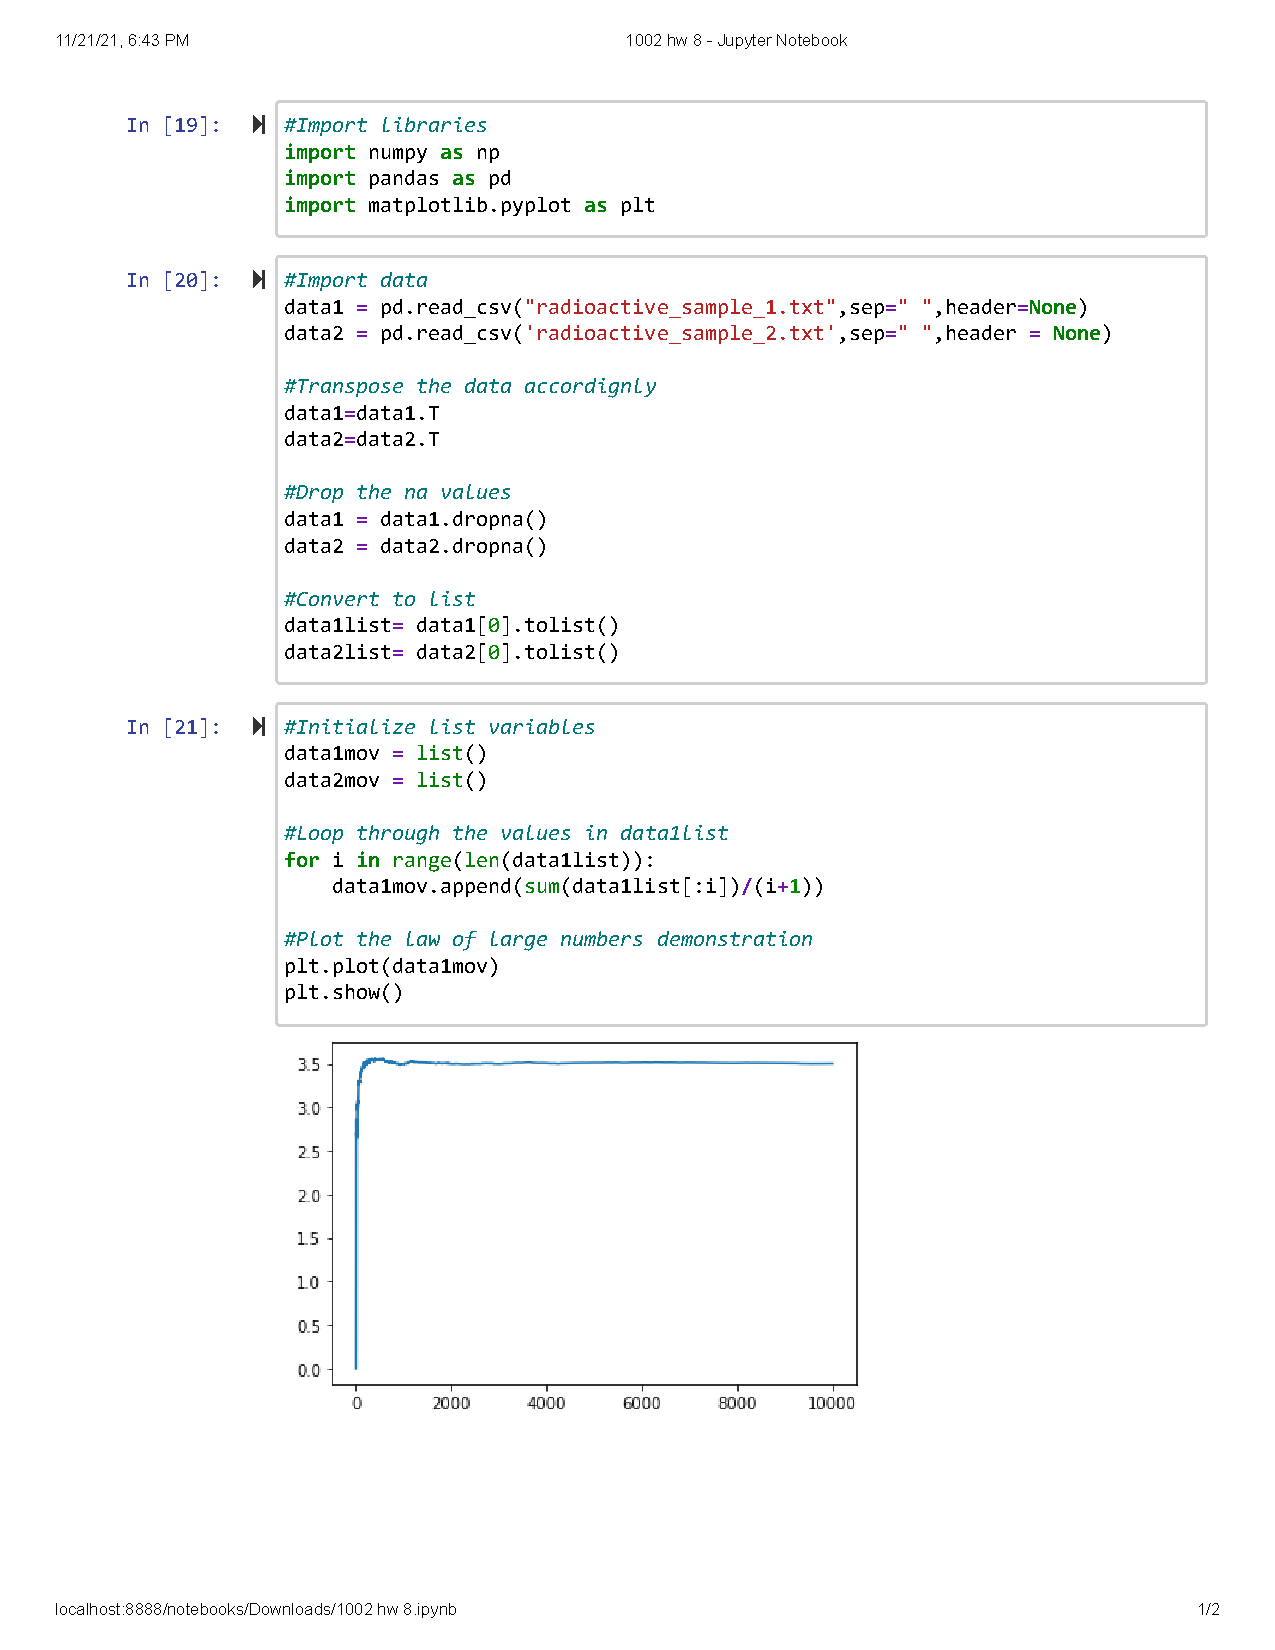
\includepdf[pages=-]{code.pdf}

\end{document}
